% replace all text with your own text.
% in this template few examples are mention
\chapter{Methodology}
\label{ch:method} % Label for method chapter

This chapter outlines the methodology used to analyse and compare the environmental impact of electric and petrol cars.
 Although electric vehicles (EVs) are often perceived as environmentally friendly,
 this study aims to demonstrate that they also contribute to pollution, although in different ways.
 The focus is on lifecycle emissions, including battery production, electricity generation, and fuel consumption.

A data analysis approach was adopted, using real-world datasets from
reputable sources such as the UK Government and the European Union \href{https://www.gov.uk/co2-and-vehicle-tax-tools}{(Government Digital Service, 2012)} . Previous studies have focused primarily on CO$_2$ emissions and air pollution caused by petrol cars, highlighting their impact on climate change.
 However, fewer studies have addressed the environmental costs of battery production and electric vehicle consumption.

To provide a balanced comparison, this study examines
CO$_2$ emissions per mile, energy consumption, and impact on the life cycle of both vehicle types.
Data preprocessing and analysis are performed using Python, while visualization tools such
as Tableau are used to present key findings. 

The methodology of this study follows a structured, systematic process to ensure the accuracy, reliability, and comprehensiveness of data analysis and visualization. The approach is divided into distinct phases, each designed to build upon the previous step, facilitating a clear and logical progression toward answering the research question

\section{Data Collection}
This is the first step, involves gathering relevant dataset that provides insights into vehicle emissions, battery production impact, and energy consumption. To ensure data reliability, the sources are carefully selected from different well-known organizations. Figure ~\ref{fig:chart_1}
\begin{lstlisting}[language=Python, caption={Code snippet in \LaTeX ~and  this is a Python code }, label=list:python_code_ex]
import pandas as pd

df = pd.read_csv("latestEuro6.csv", encoding="ISO-8859-1")


#show all columns
print(df.columns)
\end{lstlisting}
\begin{figure}[H]
    \centering
    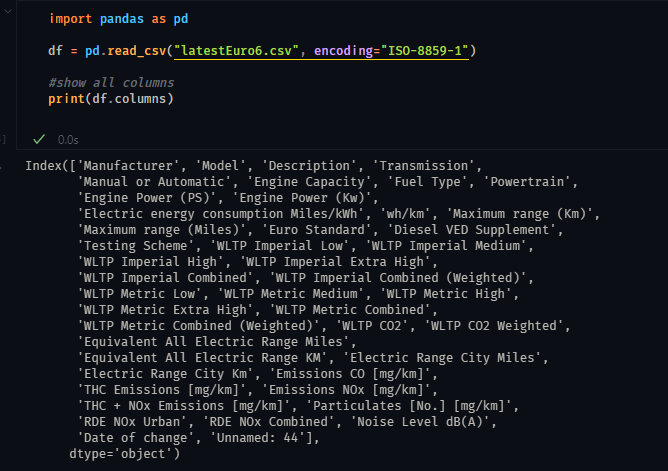
\includegraphics[scale=0.85]{figures/ColumnNames.png}
    \caption{Snapshot Column Names \LaTeX.}
    \label{fig:chart_1}
\end{figure}

Firstly, the dataset it is not being yet clean from unnecessary data, Figure ~\ref{list:python_code_list}

\begin{lstlisting}[language=Python, caption={Code snippet in \LaTeX ~and  this is a Python code, removind unnesesary data }, label=list:python_code_list]
import pandas as pd

df = pd.read_csv("latestEuro6-copy.csv", encoding="ISO-8859-1")

df = df.drop(
    columns=[
        "Model",
        "Description",
        "Transmission",
        "Manual or Automatic",
        "Powertrain",
        "Maximum range (Km)",
        "Maximum range (Miles)",
        "Euro Standard",
        "Diesel VED Supplement",
        "Testing Scheme",
        "WLTP Imperial Low",
        "WLTP Imperial Medium",
        "WLTP Imperial High",
        "WLTP Imperial Extra High",
        "WLTP Imperial Combined",
        "WLTP Imperial Combined (Weighted)",
        "WLTP Metric Low",
        "WLTP Metric Medium",
        "WLTP Metric High",
        "WLTP Metric Extra High",
        "WLTP Metric Combined",
        "WLTP Metric Combined (Weighted)",
        "WLTP CO2",
        "WLTP CO2 Weighted",
        "Equivalent All Electric Range Miles",
        "Equivalent All Electric Range KM",
        "Electric Range City Miles",
        "Electric Range City Km",
        "Emissions NOx [mg/km]",
        "THC + NOx Emissions [mg/km]",
        "Particulates [No.] [mg/km]",
        "RDE NOx Urban",
        "RDE NOx Combined",
        "Date of change",
        "Unnamed: 44",
    ]
)

\end{lstlisting}





% \begin{table}[h!]
%     \centering
%     \caption{Undergraduate report template structure}
%     \label{tab:gen_template}
%     \begin{tabular}{llll}     
%         \toprule
%         \multirow{7}{3cm}{Frontmatter} 
%         & & Title Page & \\                  
%         & & Abstract &    \\          
%         & & Acknowledgements & \\                            
%         & & Table of Contents &    \\                                
%         & & List of Figures   &    \\                        
%         & & List of Tables    &    \\                
%         & & List of Abbreviations  &    \\                     
%         & &   &    \\                        
%         \multirow{7}{3cm}{Main text}
%         & Chapter 1 & Introduction   &    \\                         
%         & Chapter 2 & Literature Review   &    \\
%         & Chapter 3 & Methodology   &    \\
%         & Chapter 4 & Results    &    \\
%         & Chapter 5 & Discussion and Analysis  &    \\
%         & Chapter 6 & Conclusions and Future Work  &    \\        
%         & Chapter 7 & Refection  &    \\          
%         & &   &    \\                       
%         \multirow{2}{3cm}{End matter}
%         & & References  &    \\   
%         & & Appendices (Optional)  &    \\ 
%         & & Index (Optional)  &    \\ 
%         \bottomrule
%     \end{tabular}
% \end{table}

% % \begin{table}[h!]
% %     \centering
% %     \caption{Example of a software engineering-type report structure}
% %     \label{tab:soft_eng_temp}
% %     \begin{tabular}{lll}     
% %         \toprule                   
% %         Chapter 1 & Introduction   &    \\        
% %         Chapter 2 & Literature Review  &    \\                   
% %         Chapter 3 & Methodology   &    \\
% %         &               & Requirements specifications   \\
% %         &               & Analysis   \\
% %         &               & Design   \\
% %         &               & Implementations   \\
% %         Chapter 4 & Testing and Validation  &    \\
% %         Chapter 5 & Results and Discussion      &    \\
% %         Chapter 6 & Conclusions and Future Work  &    \\        
% %         Chapter 7 & Reflection  &    \\                          
% %         \bottomrule
% %     \end{tabular}
% % \end{table}

% \begin{table}[h!]
%     \centering
%     \caption{Example of an algorithm analysis type report structure}
%     \label{tab:algo_temp}
%     \begin{tabular}{lll}     
%         \toprule                   
%         Chapter 1 & Introduction  &    \\        
%         Chapter 2 & Literature Review  &    \\                
%         Chapter 3 & Methodology   &    \\
%         &               & Algorithms descriptions  \\
%         &               & Implementations   \\
%         &               & Experiments design   \\
%         Chapter 4 & Results       &  \\
%         Chapter 5 & Discussion and Analysis  &    \\
%         Chapter 6 & Conclusion and Future Work  &    \\        
%         Chapter 7 & Reflection  &    \\          
%         \bottomrule
%     \end{tabular}
% \end{table}

% \begin{table}[h!]
%     \centering
%     \caption{Example of an application type report structure}
%     \label{tab:app_temp}
%     \begin{tabular}{lll}     
%         \toprule                   
%         Chapter 1 & Introduction  &    \\        
%         Chapter 2 & Literature Review  &    \\                
%         Chapter 3 & Methodology   &    \\
%         &               & Problems (tasks) descriptions  \\
%         &               & Algorithms/tools/technologies/etc. descriptions  \\        
%         &               & Implementations   \\
%         &               & Experiments design and setup   \\
%         Chapter 4 & Results       &  \\
%         Chapter 5 & Discussion and Analysis  &    \\
%         Chapter 6 & Conclusion and Future Work  &    \\        
%         Chapter 7 & Reflection  &    \\          
%         \bottomrule
%     \end{tabular}
% \end{table}

% \begin{table}[h!]
%     \centering
%     \caption{Example of a science lab experiment-type report structure}
%     \label{tab:lab_temp}
%     \begin{tabular}{lll}     
%         \toprule                   
%         Chapter 1 & Introduction  &    \\        
%         Chapter 2 & Literature Review  &    \\                
%         Chapter 3 & Materials and Methods   &    \\
%         &               & Problems (tasks) description  \\
%         &               & Materials \\        
%         &               & Procedures  \\                
%         &               & Implementations   \\
%         &               & Experiment set-up   \\
%         Chapter 4 & Results       &  \\
%         Chapter 5 & Discussion and Analysis  &    \\
%         Chapter 6 & Conclusion and Future Work  &    \\        
%         Chapter 7 & Reflection  &    \\          
%         \bottomrule
%     \end{tabular}
% \end{table}

% \section{Example of an Equation in \LaTeX}
% Eq.~\ref{eq:eq_example} [note that this is an example of an equation's in-text citation] is an example of an equation in \LaTeX. In Eq.~\eqref{eq:eq_example}, $ s $ is the mean of elements $ x_i \in \mathbf{x} $: 

% \begin{equation}
% \label{eq:eq_example} % label used to refer the eq in text
% s = \frac{1}{N} \sum_{i = 1}^{N} x_i. 
% \end{equation}

% Have you noticed that all the variables of the equation are defined using the \textbf{in-text} maths command \$.\$, and Eq.~\eqref{eq:eq_example} is treated as a part of the sentence with proper punctuation? Always treat an equation or expression as a part of the sentence. 

\section{Example of a Figure in \LaTeX}
Figure~\ref{fig:chart_a} is an example of a figure in \LaTeX. For more details, check the link:

\href{https://en.wikibooks.org/wiki/LaTeX/Floats,_Figures_and_Captions}{wikibooks.org/wiki/LaTeX/Floats,\_Figures\_and\_Captions}.

\noindent
Keep your artwork (graphics, figures, illustrations) clean and readable. At least 300dpi is a good resolution of a PNG format artwork. However, an SVG format artwork saved as a PDF will produce the best quality graphics. There are numerous tools out there that can produce vector graphics and let you save that as an SVG file and/or as a PDF file. One example of such a tool is the ``Flow algorithm software''. Here is the link for that: \href{http://www.flowgorithm.org/download/}{flowgorithm.org}.
\begin{figure}[ht]
    \centering
    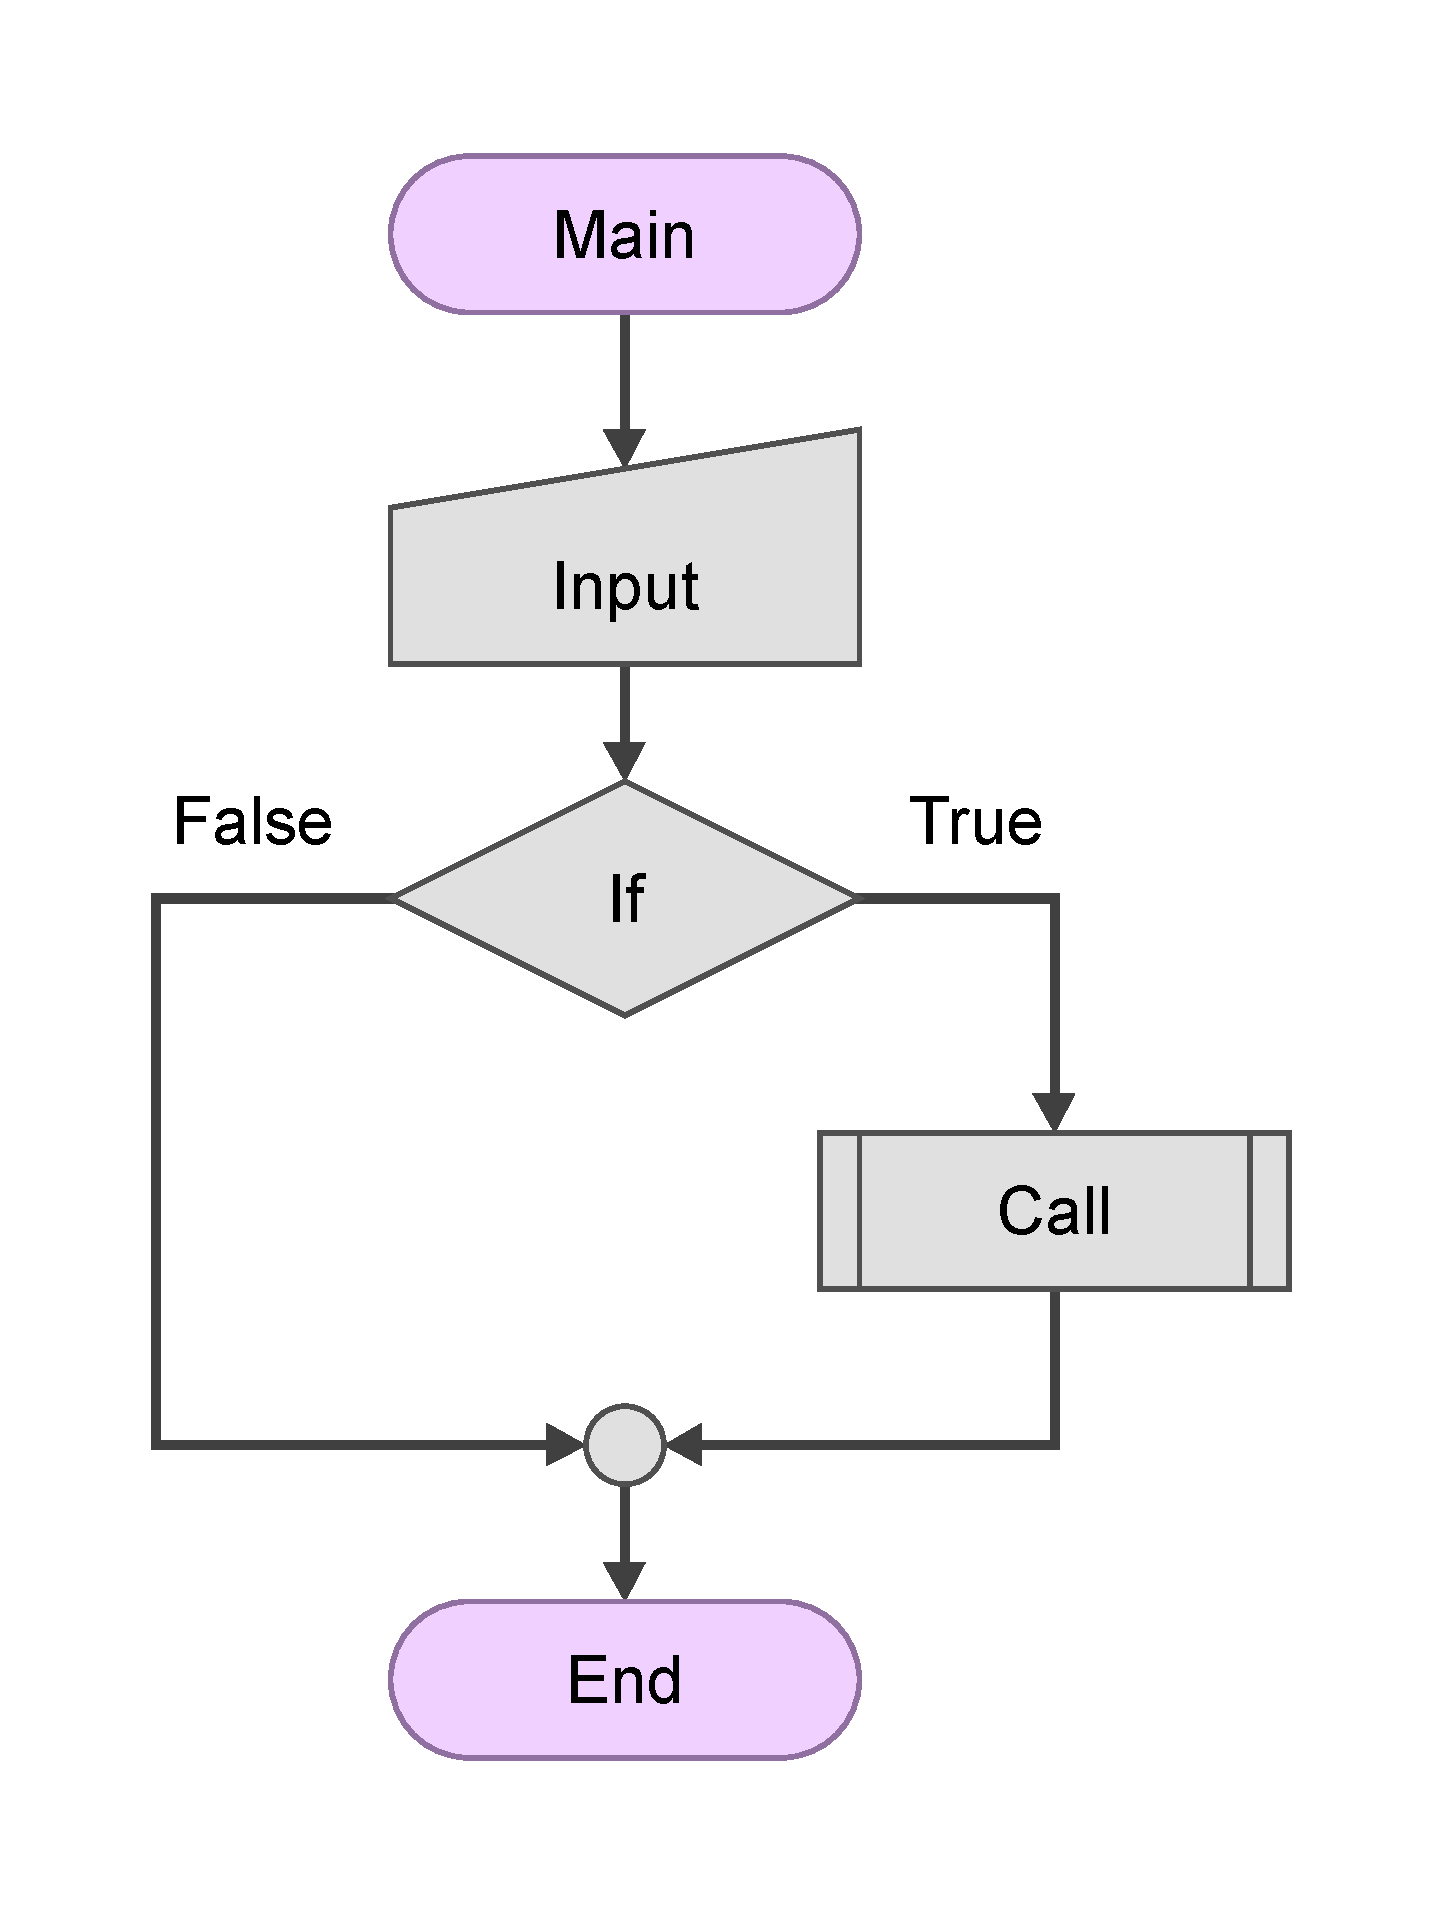
\includegraphics[scale=0.3]{figures/chart.pdf}
    \caption{Example figure in \LaTeX.}
    \label{fig:chart_a}
\end{figure}

\clearpage %  use command \clearpage when you want section or text to appear in the next page.

\section{Example of an algorithm in \LaTeX}
Algorithm~\ref{algo:algo_example} is a good example of an algorithm in \LaTeX.  
\begin{algorithm}
    \caption{Example caption: sum of all even numbers}
    \label{algo:algo_example}
    \begin{algorithmic}[1]
        \Require{$ \mathbf{x}  = x_1, x_2, \ldots, x_N$}
        \Ensure{$EvenSum$ (Sum of even numbers in $ \mathbf{x} $)}
        \Statex
        \Function{EvenSummation}{$\mathbf{x}$}
        \State {$EvenSum$ $\gets$ {$0$}}
        \State {$N$ $\gets$ {$length(\mathbf{x})$}}
        \For{$i \gets 1$ to $N$}                    
        \If{$ x_i\mod 2 == 0$}  \Comment check if a number is even?
        \State {$EvenSum$ $\gets$ {$EvenSum + x_i$}}
        \EndIf
        \EndFor
        \State \Return {$EvenSum$}
        \EndFunction
    \end{algorithmic}
\end{algorithm}
 
\section{Example of code snippet  in \LaTeX}

Code Listing~\ref{list:python_code_ex} is a good example of including a code snippet in a report. While using code snippets, take care of the following:
\begin{itemize}
    \item do not paste your entire code (implementation) or everything you have coded. Add code snippets only. 
    \item The algorithm shown in Algorithm~\ref{algo:algo_example} is usually preferred over code snippets in a technical/scientific report. 
    \item Make sure the entire code snippet or algorithm stays on a single page and does not overflow to another page(s).  
\end{itemize}

Here are three examples of code snippets for three different languages (Python, Java, and CPP) illustrated in Listings~\ref{list:python_code_ex}, \ref{list:java_code_ex}, and \ref{list:cpp_code_ex} respectively.  

\begin{lstlisting}[language=Python, caption={Code snippet in \LaTeX ~and  this is a Python code example}, label=list:python_code_ex]
import numpy as np

x  = [0, 1, 2, 3, 4, 5] # assign values to an array
evenSum = evenSummation(x) # call a function

def evenSummation(x):
    evenSum = 0
    n = len(x)
    for i in range(n):
        if np.mod(x[i],2) == 0: # check if a number is even?
            evenSum = evenSum + x[i]
    return evenSum
\end{lstlisting}

Here we used  the ``\textbackslash clearpage'' command and forced-out the second listing example onto the next page. 
\clearpage  %
\begin{lstlisting}[language=Java, caption={Code snippet in \LaTeX ~and  this is a Java code example}, label=list:java_code_ex]
public class EvenSum{ 
    public static int evenSummation(int[] x){
        int evenSum = 0;
        int n = x.length;
        for(int i = 0; i < n; i++){
            if(x[i]%2 == 0){ // check if a number is even?
                evenSum = evenSum + x[i];
            }
        }
        return evenSum;     
    }
    public static void main(String[] args){ 
        int[] x  = {0, 1, 2, 3, 4, 5}; // assign values to an array
        int evenSum = evenSummation(x);
        System.out.println(evenSum);
    } 
} 
\end{lstlisting}


\begin{lstlisting}[language=C, caption={Code snippet in \LaTeX ~and  this is a C/C++ code example}, label=list:cpp_code_ex]
int evenSummation(int x[]){
    int evenSum = 0;
    int n = sizeof(x);
    for(int i = 0; i < n; i++){
        if(x[i]%2 == 0){ // check if a number is even?
            evenSum = evenSum + x[i];
    	}
    }
    return evenSum;     
}

int main(){
    int x[]  = {0, 1, 2, 3, 4, 5}; // assign values to an array
    int evenSum = evenSummation(x);
    cout<<evenSum;
    return 0;
}
\end{lstlisting}



\section{Example of in-text citation style}
\subsection{Example of the equations and illustrations placement and reference in the text}
Make sure whenever you refer to the equations, tables, figures, algorithms,  and listings for the first time, they also appear (placed) somewhere on the same page or in the following page(s). Always make sure to refer to the equations, tables and figures used in the report. Do not leave them without an \textbf{in-text citation}. You can refer to equations, tables and figures more them once.

\subsection{Example of the equations and illustrations style}
Write \textbf{Eq.} with an uppercase ``Eq`` for an equation before using an equation number with (\textbackslash eqref\{.\}). Use ``Table'' to refer to a table, ``Figure'' to refer to a figure, ``Algorithm'' to refer to an algorithm and ``Listing'' to refer to listings (code snippets). Note that, we do not use the articles ``a,'' ``an,'' and ``the'' before the words Eq., Figure, Table, and Listing, but you may use an article for referring the words figure, table, etc. in general.

For example, the sentence ``A report structure is shown in \textbf{the} Table~\ref{tab:gen_template}'' should be written as ``A report structure is shown \textbf{in} Table~\ref{tab:gen_template}.'' 
 

\section{Summary}
Write a summary of this chapter.

~\\[5em]
\noindent
{\huge\textbf{Note:}} In the case of \textbf{software engineering} project a Chapter ``\textbf{Testing and Validation}'' should precede the ``Results'' chapter. See Section~\ref{subsec:se_chpters} for report organization of such project. 

